\documentclass[border=6pt]{standalone}
% Shared preamble for web figures.  Each figure is a standalone .tex that
% \input's this file; scripts/make-figures.sh turns it into an SVG.
\usepackage[T1]{fontenc}
\usepackage{helvet}
\renewcommand{\familydefault}{\sfdefault}
\usepackage{tikz}
\usetikzlibrary{decorations.pathreplacing}
% axis numbers in the text font, not math italic
\pgfkeys{/pgf/number format/.cd,assume math mode=true,1000 sep={}}

% dot plot: \dotplot{min}{max}{value/count,...}{axis label}
\newcommand{\dotplot}[4]{%
\begin{tikzpicture}[x=0.9cm,y=0.33cm]
  \draw[thick] (#1-0.5,0) -- (#2+0.5,0);
  \foreach \t in {#1,...,#2} {\draw (\t,0.25) -- (\t,-0.25) node[below] {\t};}
  \foreach \v/\c in {#3} {\ifnum\c>0 \foreach \k in {1,...,\c} {\fill (\v,\k*1.15) circle (0.16cm);}\fi}
  \node at ({(#1+#2)/2},-2.3) {#4};
\end{tikzpicture}}

% shape sketch histogram (12 bins): \shapehist{heights}{label}
\newcommand{\shapehist}[2]{%
  \foreach \h [count=\i from 0] in {#1} \draw[fill=gray!30] (\i,0) rectangle (\i+1,\h);
  \draw (-0.3,0) -- (12.3,0);
  \node[font=\bfseries] at (6,-2.6) {#2};}
\newcommand{\meanmark}[1]{\fill (#1,0) -- ++(-0.3,-0.75) -- ++(0.6,0) -- cycle;}
\newcommand{\medmark}[2]{\draw[very thick,dashed] (#1,0) -- (#1,#2);}

% number line with minor ticks: \nline{min}{max}{label step}{axis label}
\newcommand{\nline}[4]{%
  \draw[thick] (#1-0.5,0) -- (#2+0.5,0);
  \foreach \t in {#1,...,#2} \draw (\t,0.12) -- (\t,-0.12);
  \pgfmathtruncatemacro{\nxt}{#1+#3}
  \foreach \t in {#1,\nxt,...,#2} \draw (\t,0.2) -- (\t,-0.2) node[below] {\t};
  \node at ({(#1+#2)/2},-0.95) {#4};}
% box plot above the line: \bplot{min}{Q1}{med}{Q3}{max}
\newcommand{\bplot}[5]{%
  \draw[thick] (#1,1.0) -- (#2,1.0);
  \draw[thick] (#4,1.0) -- (#5,1.0);
  \draw[thick] (#1,0.75) -- (#1,1.25);
  \draw[thick] (#5,0.75) -- (#5,1.25);
  \draw[thick,fill=gray!20] (#2,0.55) rectangle (#4,1.45);
  \draw[very thick] (#3,0.55) -- (#3,1.45);}

% ---- added for 1.4 onward ----
% axis on y=0: \axis{min}{max}{label step}{tick step}{axis label}
\newcommand{\axis}[5]{%
  \draw[thick] (#1,0) -- (#2,0);
  \pgfmathsetmacro{\axT}{#1+#4}\foreach \t in {#1,\axT,...,#2} \draw (\t,0.1) -- (\t,-0.1);
  \pgfmathsetmacro{\axL}{#1+#3}\foreach \t in {#1,\axL,...,#2}
    \draw (\t,0.18) -- (\t,-0.18) node[below] {\pgfmathprintnumber{\t}};
  \node at ({(#1+#2)/2},-0.95) {#5};}
% box plot centred at height y: \bplotat{y}{min}{Q1}{med}{Q3}{max}
\newcommand{\bplotat}[6]{%
  \draw[thick] (#2,#1) -- (#3,#1);
  \draw[thick] (#5,#1) -- (#6,#1);
  \draw[thick] (#2,#1-0.22) -- (#2,#1+0.22);
  \draw[thick] (#6,#1-0.22) -- (#6,#1+0.22);
  \draw[thick,fill=gray!20] (#3,#1-0.42) rectangle (#5,#1+0.42);
  \draw[very thick] (#4,#1-0.42) -- (#4,#1+0.42);}
% an outlier dot: \outlier{x}{y}
\newcommand{\outlier}[2]{\fill (#1,#2) circle (2.4pt);}

\begin{document}
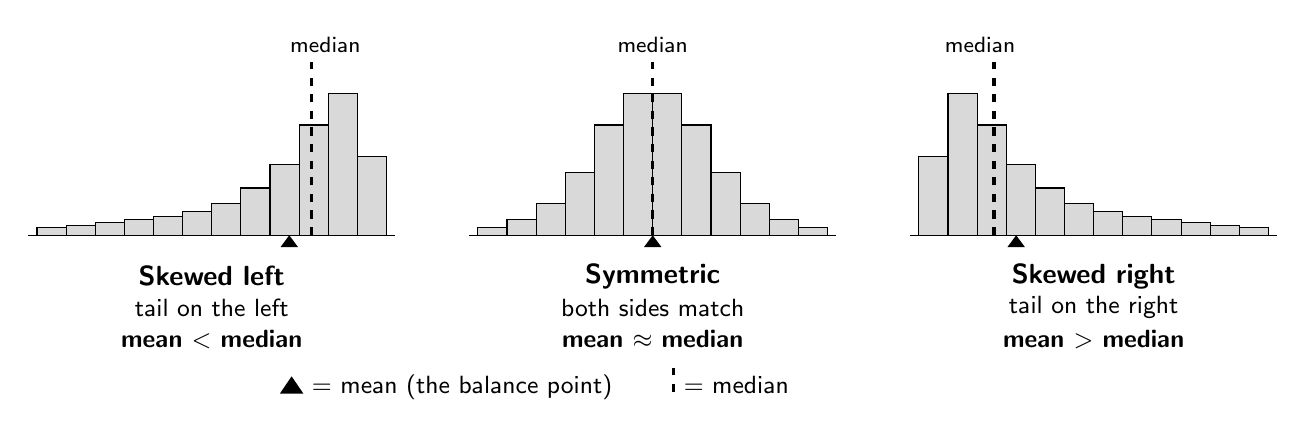
\begin{tikzpicture}[x=0.37cm,y=0.2cm]
\begin{scope}
  \shapehist{0.5,0.6,0.8,1,1.2,1.5,2,3,4.5,7,9,5}{Skewed left}
  \medmark{9.42}{11} \meanmark{8.66}
  \node[font=\footnotesize,anchor=south] at (9.9,11) {median};
  \node[font=\small] at (6,-4.6) {tail on the left};
  \node[font=\small] at (6,-6.6) {\textbf{mean $<$ median}};
\end{scope}
\begin{scope}[xshift=5.6cm]
  \shapehist{0.5,1,2,4,7,9,9,7,4,2,1,0.5}{Symmetric}
  \medmark{6}{11} \meanmark{6}
  \node[font=\footnotesize,anchor=south] at (6,11) {median};
  \node[font=\small] at (6,-4.6) {both sides match};
  \node[font=\small] at (6,-6.6) {\textbf{mean $\approx$ median}};
\end{scope}
\begin{scope}[xshift=11.2cm]
  \shapehist{5,9,7,4.5,3,2,1.5,1.2,1,0.8,0.6,0.5}{Skewed right}
  \medmark{2.58}{11} \meanmark{3.34}
  \node[font=\footnotesize,anchor=south] at (2.1,11) {median};
  \node[font=\small] at (6,-4.6) {tail on the right};
  \node[font=\small] at (6,-6.6) {\textbf{mean $>$ median}};
\end{scope}
\node[font=\small,anchor=west] at (8,-9.4) {\tikz[x=1cm,y=1cm]\fill (0,0) -- (0.3,0) -- (0.15,0.22) -- cycle; = mean (the balance point) \qquad \tikz[x=1cm,y=1cm]\draw[very thick,dashed] (0,0) -- (0,0.3); = median};
\end{tikzpicture}
\end{document}
